% Created by tikzDevice version 0.12.6 on 2024-09-23 08:23:22
% !TEX encoding = UTF-8 Unicode
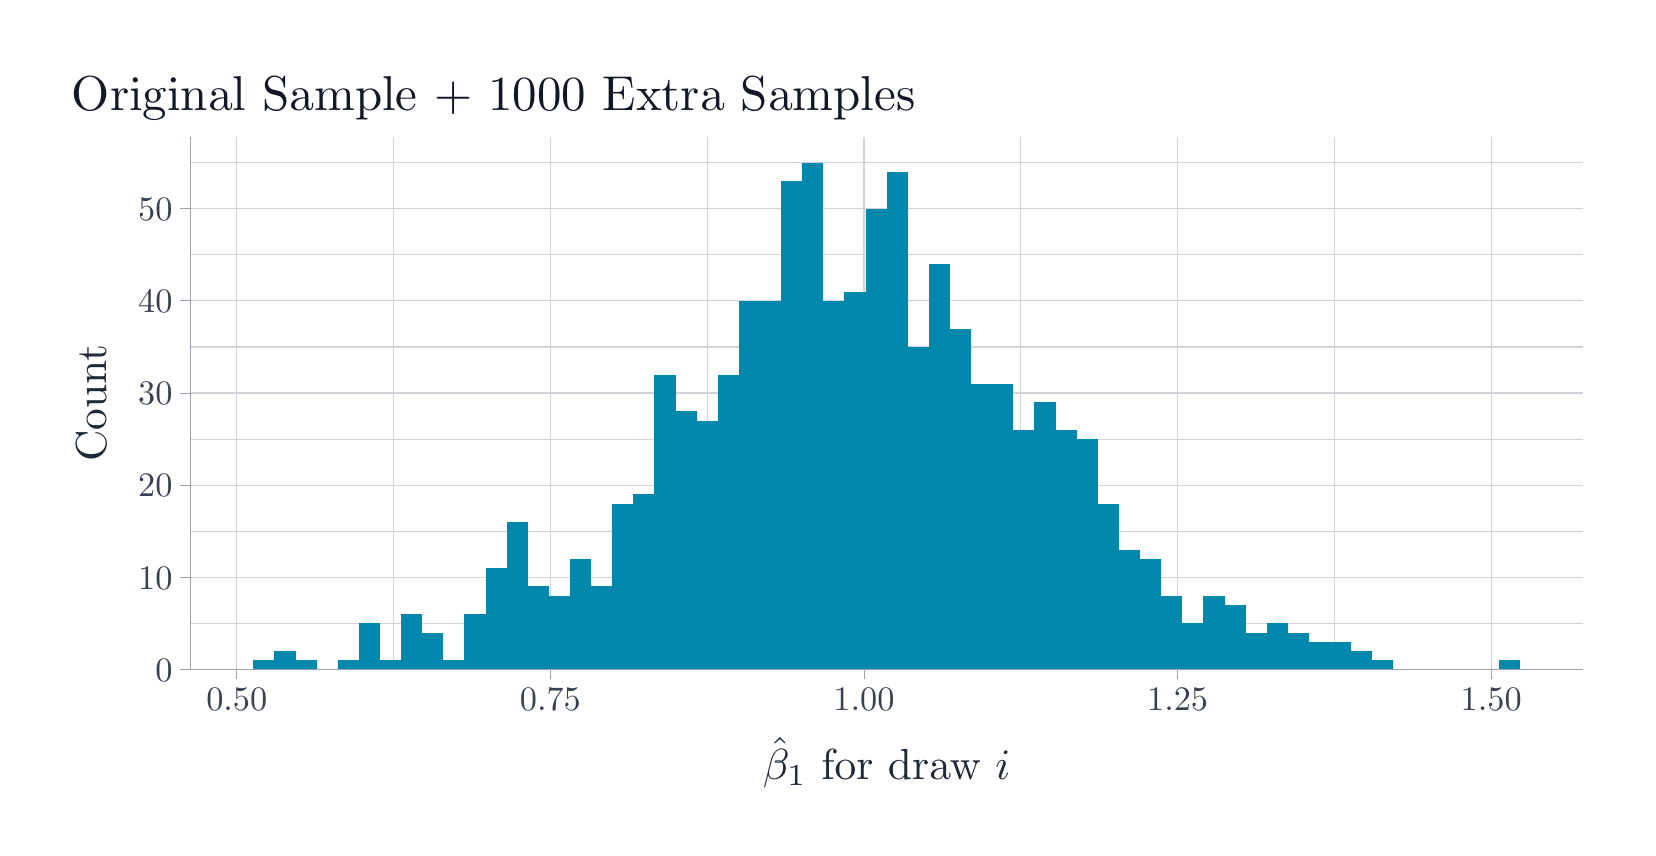
\begin{tikzpicture}[x=1pt,y=1pt]
\definecolor{fillColor}{RGB}{255,255,255}
\path[use as bounding box,fill=fillColor] (0,0) rectangle (578.16,289.08);
\begin{scope}
\path[clip] (  0.00,  0.00) rectangle (578.16,289.08);
\definecolor{drawColor}{RGB}{255,255,255}

\path[draw=drawColor,line width= 0.7pt,line join=round,line cap=round,fill=fillColor] (  0.00,  0.00) rectangle (578.16,289.08);
\end{scope}
\begin{scope}
\path[clip] ( 58.65, 57.20) rectangle (562.16,249.43);
\definecolor{drawColor}{RGB}{255,255,255}
\definecolor{fillColor}{RGB}{255,255,255}

\path[draw=drawColor,line width= 0.7pt,line join=round,line cap=round,fill=fillColor] ( 58.65, 57.20) rectangle (562.16,249.43);
\definecolor{drawColor}{RGB}{209,213,219}

\path[draw=drawColor,line width= 0.4pt,line join=round] ( 58.65, 73.84) --
	(562.16, 73.84);

\path[draw=drawColor,line width= 0.4pt,line join=round] ( 58.65,107.13) --
	(562.16,107.13);

\path[draw=drawColor,line width= 0.4pt,line join=round] ( 58.65,140.41) --
	(562.16,140.41);

\path[draw=drawColor,line width= 0.4pt,line join=round] ( 58.65,173.70) --
	(562.16,173.70);

\path[draw=drawColor,line width= 0.4pt,line join=round] ( 58.65,206.99) --
	(562.16,206.99);

\path[draw=drawColor,line width= 0.4pt,line join=round] ( 58.65,240.28) --
	(562.16,240.28);

\path[draw=drawColor,line width= 0.4pt,line join=round] (132.22, 57.20) --
	(132.22,249.43);

\path[draw=drawColor,line width= 0.4pt,line join=round] (245.54, 57.20) --
	(245.54,249.43);

\path[draw=drawColor,line width= 0.4pt,line join=round] (358.87, 57.20) --
	(358.87,249.43);

\path[draw=drawColor,line width= 0.4pt,line join=round] (472.19, 57.20) --
	(472.19,249.43);

\path[draw=drawColor,line width= 0.4pt,line join=round] ( 58.65, 57.20) --
	(562.16, 57.20);

\path[draw=drawColor,line width= 0.4pt,line join=round] ( 58.65, 90.48) --
	(562.16, 90.48);

\path[draw=drawColor,line width= 0.4pt,line join=round] ( 58.65,123.77) --
	(562.16,123.77);

\path[draw=drawColor,line width= 0.4pt,line join=round] ( 58.65,157.06) --
	(562.16,157.06);

\path[draw=drawColor,line width= 0.4pt,line join=round] ( 58.65,190.35) --
	(562.16,190.35);

\path[draw=drawColor,line width= 0.4pt,line join=round] ( 58.65,223.63) --
	(562.16,223.63);

\path[draw=drawColor,line width= 0.4pt,line join=round] ( 75.56, 57.20) --
	( 75.56,249.43);

\path[draw=drawColor,line width= 0.4pt,line join=round] (188.88, 57.20) --
	(188.88,249.43);

\path[draw=drawColor,line width= 0.4pt,line join=round] (302.20, 57.20) --
	(302.20,249.43);

\path[draw=drawColor,line width= 0.4pt,line join=round] (415.53, 57.20) --
	(415.53,249.43);

\path[draw=drawColor,line width= 0.4pt,line join=round] (528.85, 57.20) --
	(528.85,249.43);
\definecolor{fillColor}{RGB}{1,136,172}

\path[fill=fillColor] ( 81.53, 57.20) rectangle ( 89.16, 60.52);

\path[fill=fillColor] ( 89.16, 57.20) rectangle ( 96.79, 63.85);

\path[fill=fillColor] ( 96.79, 57.20) rectangle (104.42, 60.52);

\path[fill=fillColor] (104.42, 57.20) rectangle (112.05, 57.20);

\path[fill=fillColor] (112.05, 57.20) rectangle (119.68, 60.52);

\path[fill=fillColor] (119.68, 57.20) rectangle (127.31, 73.84);

\path[fill=fillColor] (127.31, 57.20) rectangle (134.94, 60.52);

\path[fill=fillColor] (134.94, 57.20) rectangle (142.57, 77.17);

\path[fill=fillColor] (142.57, 57.20) rectangle (150.19, 70.51);

\path[fill=fillColor] (150.19, 57.20) rectangle (157.82, 60.52);

\path[fill=fillColor] (157.82, 57.20) rectangle (165.45, 77.17);

\path[fill=fillColor] (165.45, 57.20) rectangle (173.08, 93.81);

\path[fill=fillColor] (173.08, 57.20) rectangle (180.71,110.46);

\path[fill=fillColor] (180.71, 57.20) rectangle (188.34, 87.15);

\path[fill=fillColor] (188.34, 57.20) rectangle (195.97, 83.83);

\path[fill=fillColor] (195.97, 57.20) rectangle (203.60, 97.14);

\path[fill=fillColor] (203.60, 57.20) rectangle (211.23, 87.15);

\path[fill=fillColor] (211.23, 57.20) rectangle (218.86,117.11);

\path[fill=fillColor] (218.86, 57.20) rectangle (226.48,120.44);

\path[fill=fillColor] (226.48, 57.20) rectangle (234.11,163.72);

\path[fill=fillColor] (234.11, 57.20) rectangle (241.74,150.40);

\path[fill=fillColor] (241.74, 57.20) rectangle (249.37,147.07);

\path[fill=fillColor] (249.37, 57.20) rectangle (257.00,163.72);

\path[fill=fillColor] (257.00, 57.20) rectangle (264.63,190.35);

\path[fill=fillColor] (264.63, 57.20) rectangle (272.26,190.35);

\path[fill=fillColor] (272.26, 57.20) rectangle (279.89,233.62);

\path[fill=fillColor] (279.89, 57.20) rectangle (287.52,240.28);

\path[fill=fillColor] (287.52, 57.20) rectangle (295.15,190.35);

\path[fill=fillColor] (295.15, 57.20) rectangle (302.77,193.67);

\path[fill=fillColor] (302.77, 57.20) rectangle (310.40,223.63);

\path[fill=fillColor] (310.40, 57.20) rectangle (318.03,236.95);

\path[fill=fillColor] (318.03, 57.20) rectangle (325.66,173.70);

\path[fill=fillColor] (325.66, 57.20) rectangle (333.29,203.66);

\path[fill=fillColor] (333.29, 57.20) rectangle (340.92,180.36);

\path[fill=fillColor] (340.92, 57.20) rectangle (348.55,160.39);

\path[fill=fillColor] (348.55, 57.20) rectangle (356.18,160.39);

\path[fill=fillColor] (356.18, 57.20) rectangle (363.81,143.74);

\path[fill=fillColor] (363.81, 57.20) rectangle (371.44,153.73);

\path[fill=fillColor] (371.44, 57.20) rectangle (379.06,143.74);

\path[fill=fillColor] (379.06, 57.20) rectangle (386.69,140.41);

\path[fill=fillColor] (386.69, 57.20) rectangle (394.32,117.11);

\path[fill=fillColor] (394.32, 57.20) rectangle (401.95,100.47);

\path[fill=fillColor] (401.95, 57.20) rectangle (409.58, 97.14);

\path[fill=fillColor] (409.58, 57.20) rectangle (417.21, 83.83);

\path[fill=fillColor] (417.21, 57.20) rectangle (424.84, 73.84);

\path[fill=fillColor] (424.84, 57.20) rectangle (432.47, 83.83);

\path[fill=fillColor] (432.47, 57.20) rectangle (440.10, 80.50);

\path[fill=fillColor] (440.10, 57.20) rectangle (447.73, 70.51);

\path[fill=fillColor] (447.73, 57.20) rectangle (455.35, 73.84);

\path[fill=fillColor] (455.35, 57.20) rectangle (462.98, 70.51);

\path[fill=fillColor] (462.98, 57.20) rectangle (470.61, 67.18);

\path[fill=fillColor] (470.61, 57.20) rectangle (478.24, 67.18);

\path[fill=fillColor] (478.24, 57.20) rectangle (485.87, 63.85);

\path[fill=fillColor] (485.87, 57.20) rectangle (493.50, 60.52);

\path[fill=fillColor] (493.50, 57.20) rectangle (501.13, 57.20);

\path[fill=fillColor] (501.13, 57.20) rectangle (508.76, 57.20);

\path[fill=fillColor] (508.76, 57.20) rectangle (516.39, 57.20);

\path[fill=fillColor] (516.39, 57.20) rectangle (524.02, 57.20);

\path[fill=fillColor] (524.02, 57.20) rectangle (531.64, 57.20);

\path[fill=fillColor] (531.64, 57.20) rectangle (539.27, 60.52);
\end{scope}
\begin{scope}
\path[clip] (  0.00,  0.00) rectangle (578.16,289.08);
\definecolor{drawColor}{RGB}{156,163,175}

\path[draw=drawColor,line width= 0.3pt,line join=round] ( 58.65, 57.20) --
	( 58.65,249.43);
\end{scope}
\begin{scope}
\path[clip] (  0.00,  0.00) rectangle (578.16,289.08);
\definecolor{drawColor}{RGB}{55,65,81}

\node[text=drawColor,anchor=base east,inner sep=0pt, outer sep=0pt, scale=  1.24] at ( 52.35, 52.91) {0};

\node[text=drawColor,anchor=base east,inner sep=0pt, outer sep=0pt, scale=  1.24] at ( 52.35, 86.20) {10};

\node[text=drawColor,anchor=base east,inner sep=0pt, outer sep=0pt, scale=  1.24] at ( 52.35,119.49) {20};

\node[text=drawColor,anchor=base east,inner sep=0pt, outer sep=0pt, scale=  1.24] at ( 52.35,152.77) {30};

\node[text=drawColor,anchor=base east,inner sep=0pt, outer sep=0pt, scale=  1.24] at ( 52.35,186.06) {40};

\node[text=drawColor,anchor=base east,inner sep=0pt, outer sep=0pt, scale=  1.24] at ( 52.35,219.35) {50};
\end{scope}
\begin{scope}
\path[clip] (  0.00,  0.00) rectangle (578.16,289.08);
\definecolor{drawColor}{RGB}{156,163,175}

\path[draw=drawColor,line width= 0.3pt,line join=round] ( 55.15, 57.20) --
	( 58.65, 57.20);

\path[draw=drawColor,line width= 0.3pt,line join=round] ( 55.15, 90.48) --
	( 58.65, 90.48);

\path[draw=drawColor,line width= 0.3pt,line join=round] ( 55.15,123.77) --
	( 58.65,123.77);

\path[draw=drawColor,line width= 0.3pt,line join=round] ( 55.15,157.06) --
	( 58.65,157.06);

\path[draw=drawColor,line width= 0.3pt,line join=round] ( 55.15,190.35) --
	( 58.65,190.35);

\path[draw=drawColor,line width= 0.3pt,line join=round] ( 55.15,223.63) --
	( 58.65,223.63);
\end{scope}
\begin{scope}
\path[clip] (  0.00,  0.00) rectangle (578.16,289.08);
\definecolor{drawColor}{RGB}{156,163,175}

\path[draw=drawColor,line width= 0.3pt,line join=round] ( 58.65, 57.20) --
	(562.16, 57.20);
\end{scope}
\begin{scope}
\path[clip] (  0.00,  0.00) rectangle (578.16,289.08);
\definecolor{drawColor}{RGB}{156,163,175}

\path[draw=drawColor,line width= 0.3pt,line join=round] ( 75.56, 53.70) --
	( 75.56, 57.20);

\path[draw=drawColor,line width= 0.3pt,line join=round] (188.88, 53.70) --
	(188.88, 57.20);

\path[draw=drawColor,line width= 0.3pt,line join=round] (302.20, 53.70) --
	(302.20, 57.20);

\path[draw=drawColor,line width= 0.3pt,line join=round] (415.53, 53.70) --
	(415.53, 57.20);

\path[draw=drawColor,line width= 0.3pt,line join=round] (528.85, 53.70) --
	(528.85, 57.20);
\end{scope}
\begin{scope}
\path[clip] (  0.00,  0.00) rectangle (578.16,289.08);
\definecolor{drawColor}{RGB}{55,65,81}

\node[text=drawColor,anchor=base,inner sep=0pt, outer sep=0pt, scale=  1.24] at ( 75.56, 42.33) {0.50};

\node[text=drawColor,anchor=base,inner sep=0pt, outer sep=0pt, scale=  1.24] at (188.88, 42.33) {0.75};

\node[text=drawColor,anchor=base,inner sep=0pt, outer sep=0pt, scale=  1.24] at (302.20, 42.33) {1.00};

\node[text=drawColor,anchor=base,inner sep=0pt, outer sep=0pt, scale=  1.24] at (415.53, 42.33) {1.25};

\node[text=drawColor,anchor=base,inner sep=0pt, outer sep=0pt, scale=  1.24] at (528.85, 42.33) {1.50};
\end{scope}
\begin{scope}
\path[clip] (  0.00,  0.00) rectangle (578.16,289.08);
\definecolor{drawColor}{RGB}{31,41,55}

\node[text=drawColor,anchor=base,inner sep=0pt, outer sep=0pt, scale=  1.57] at (310.40, 17.53) {$\hat{\beta}_1$ for draw $i$};
\end{scope}
\begin{scope}
\path[clip] (  0.00,  0.00) rectangle (578.16,289.08);
\definecolor{drawColor}{RGB}{31,41,55}

\node[text=drawColor,rotate= 90.00,anchor=base,inner sep=0pt, outer sep=0pt, scale=  1.57] at ( 28.38,153.31) {Count};
\end{scope}
\begin{scope}
\path[clip] (  0.00,  0.00) rectangle (578.16,289.08);
\definecolor{drawColor}{RGB}{17,24,39}

\node[text=drawColor,anchor=base west,inner sep=0pt, outer sep=0pt, scale=  1.77] at ( 16.00,259.15) {Original Sample + 1000 Extra Samples};
\end{scope}
\end{tikzpicture}
